\renewcommand{\chaptername}{Chapter} 
\chapter{Perseveration analysis}\label{chap9}
In this chapter, we delve deeper into the posterior results obtained after fitting the GLM-HMM model to real data. Our goal is to explore whether specific parameters influence the likelihood of patients entering the perseverative state and, conversely, how their behavior differs when they do not perseverate. Additionally, we investigate whether there are notable differences between patients and controls in this posterior analysis, providing further insights into the mechanisms underlying perseveration and engagement in stimulus-driven tasks.
\section{Expected responses} 
An important aspect to investigate is whether participants' expected responses, derived from their engaged kernel (extracted after removing perseverative trials), align with their actual choices. Specifically, we assess whether the responses predicted based on the stimulus-kernel dot product from GLM-HMM differ from the responses observed when participants were in the engaged state.

To analyze this, we computed the expected response for both patients and controls and compared it to their actual choices. If the expected response matched the participant’s actual response, it was classified as correct; otherwise, it was classified as incorrect. The cumulative proportion of correct prediction is illustrated in Figure \ref{fig:ecdf_accuracy_by_trial}, where we observe an average accuracy of 46\% for patients (n=22) and 50\% for controls (n=22). This suggests that controls outperform patients by only 4\%, indicating that their responses are not significantly more aligned with the engaged kernel than those of patients.
\begin{figure}[H]
    \centering
    \includegraphics[width=16cm,height=7cm]{MainLayout/Images/chapter9/ecdf_accuracy_by_trial.jpg}
    \caption{Main Title for First Image \\ \small Subtitle for the first graphic.}
    \label{fig:accuracy_by_trial}
\end{figure}

\section{Number of identical responses} 
In addition to analyzing expected responses, we examined the number of consecutive identical responses to assess patterns of repetition in participants’ choices. This analysis helps determine whether their repetitive behaviors align with stimulus-driven decision-making or are influenced by perseverative tendencies.

By comparing the expected identical responses (i.e., those predicted based on the engaged kernel, assuming participants were applying their engaged state) to the actual identical responses (those observed in their real choices) in the engaged state, we can quantify how much their responses deviate from an optimal stimulus-driven pattern. If participants were strictly applying their engaged kernel, the number of consecutive identical responses would be determined by the structure of the stimulus rather than perseverative tendencies. However, by comparing this to their actual sequence of responses, we can evaluate the extent to which perseveration inflates repetition beyond what is expected from the engaged model.\newline
In Figure \ref{fig:actual_expected_controls}, we compare the expected number of consecutive identical responses (predicted using the engaged kernel) with the actual number of identical responses observed in participants' choices in engaged trials. To assess whether there is a significant difference between these distributions, we conducted a Kolmogorov-Smirnov test, which resulted in a non-significant difference (p = 0.88), indicating that the distributions of actual and expected identical responses are statistically similar.

\begin{figure}[H]
    \centering
    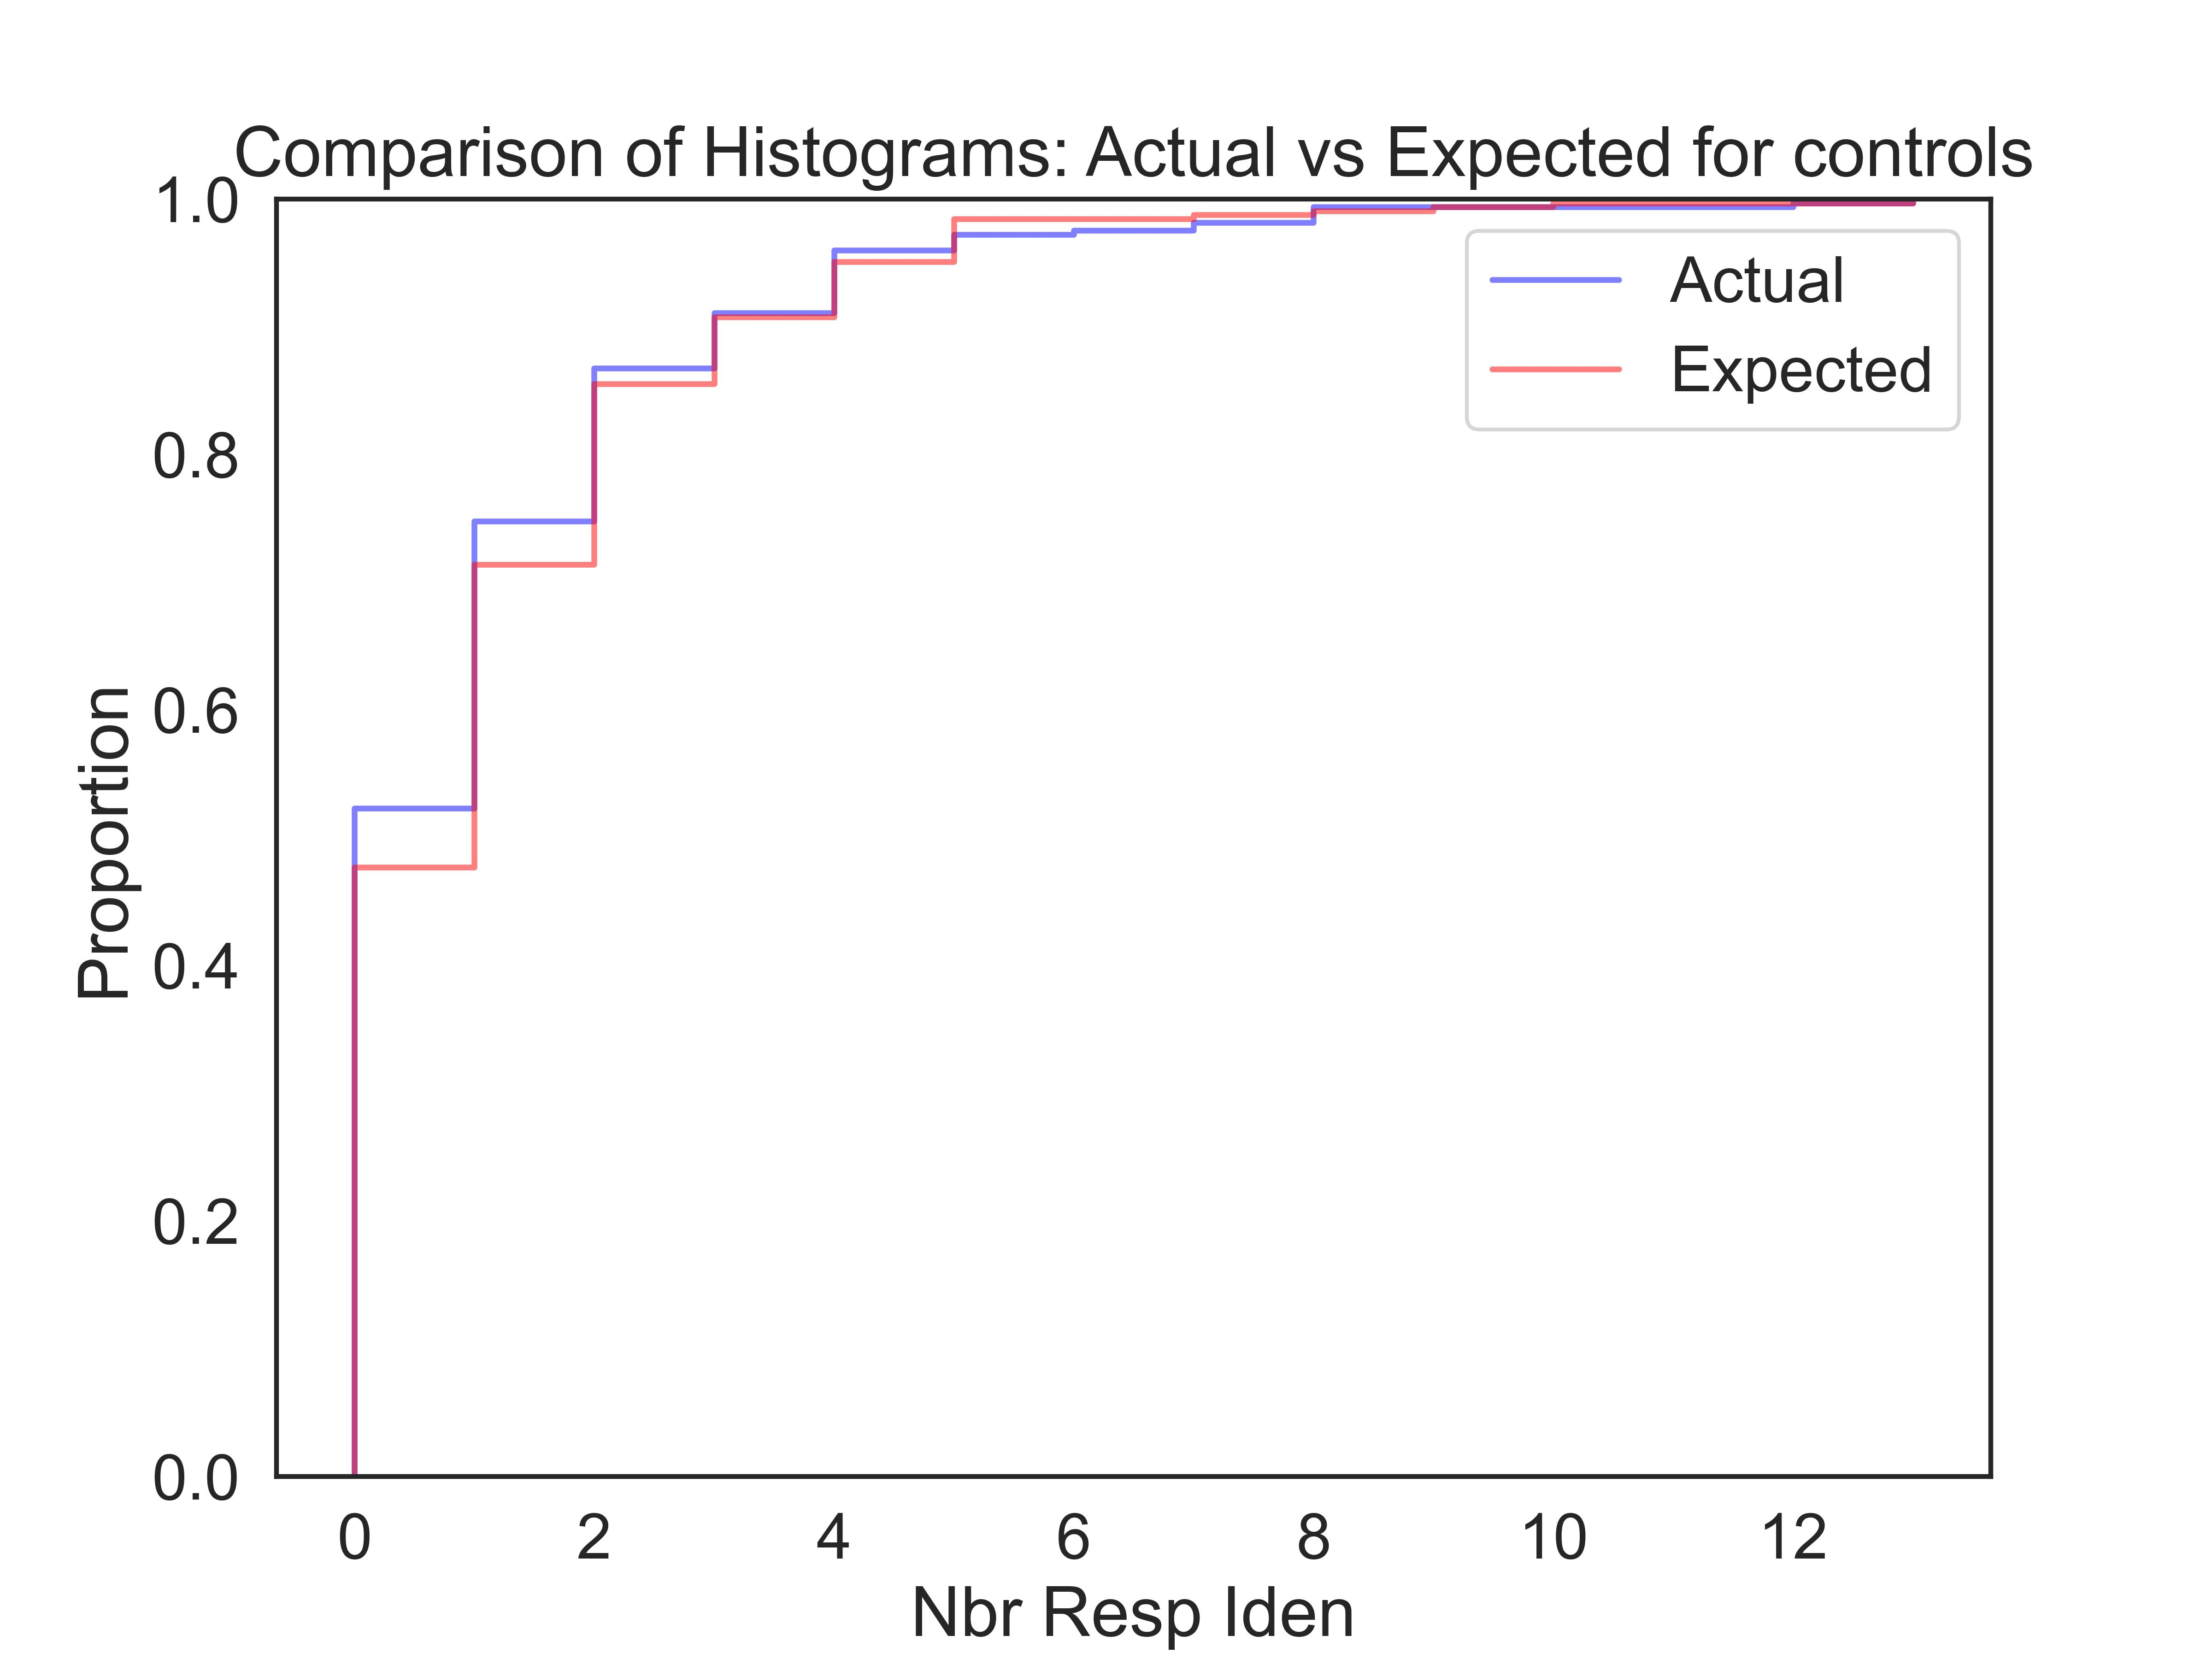
\includegraphics[width=12cm,height=7cm]{MainLayout/Images/chapter9/actual_expected_controls_ecdf.jpg}
    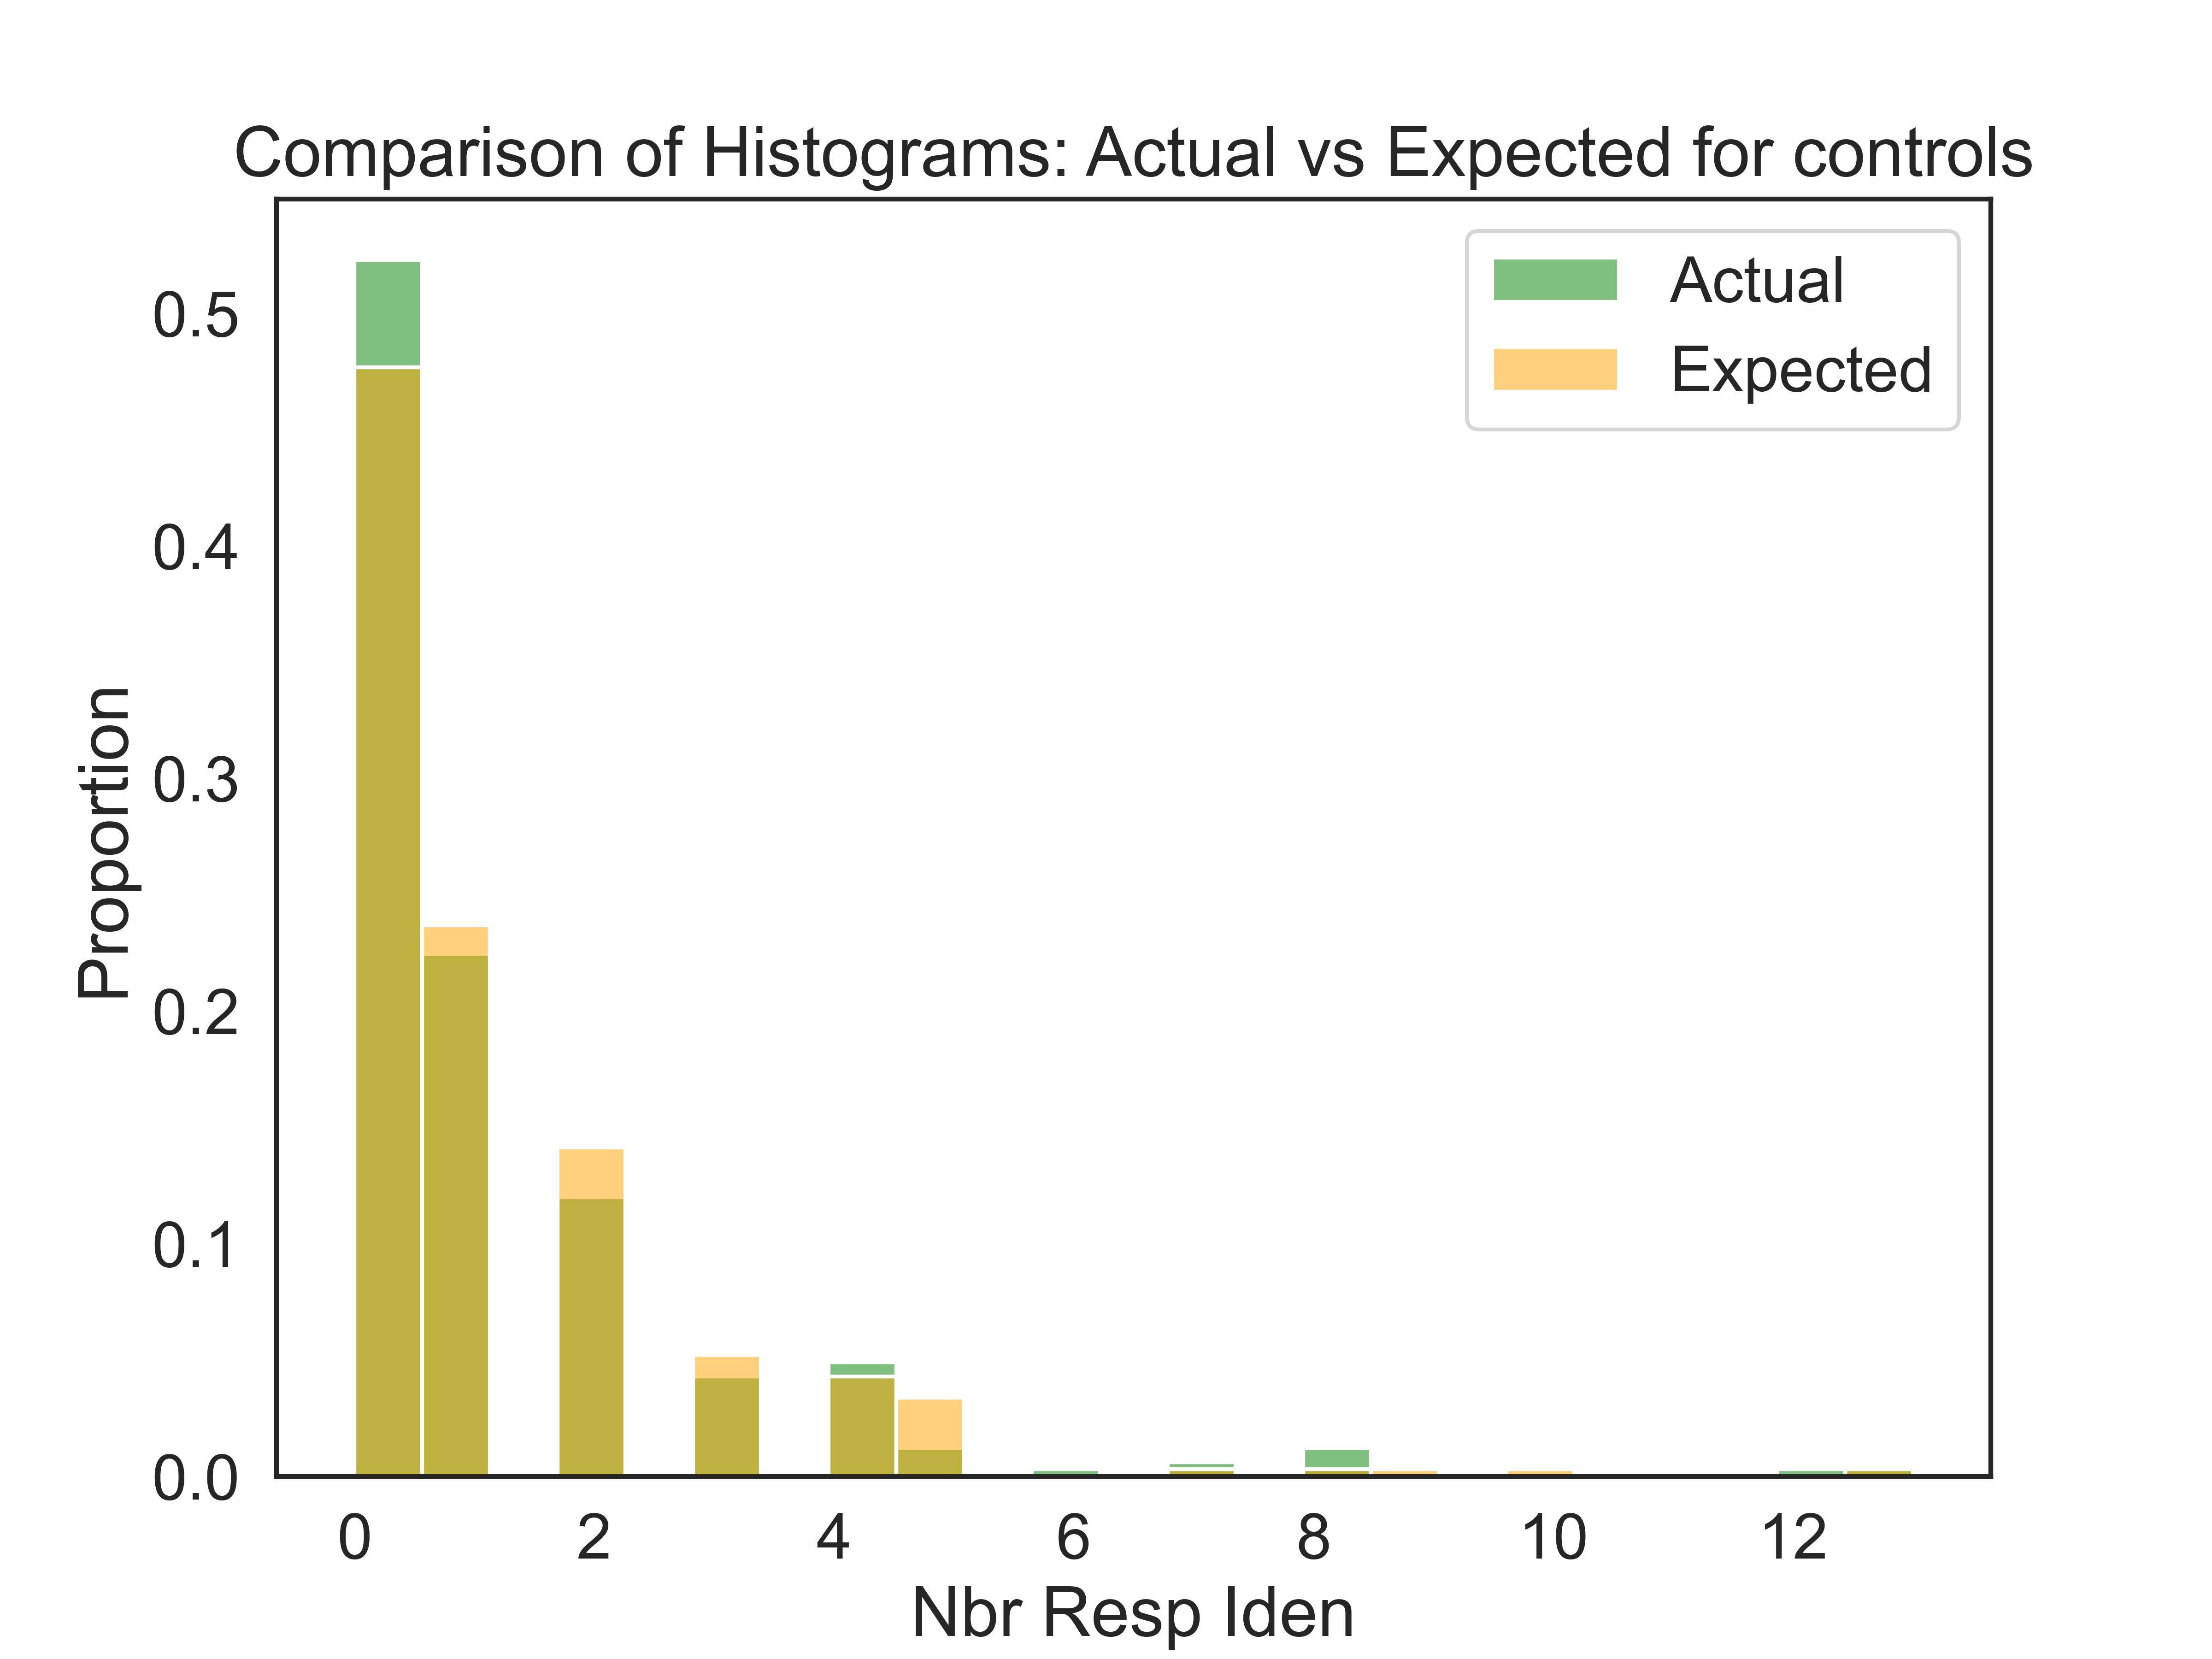
\includegraphics[width=12cm,height=7cm]{MainLayout/Images/chapter9/actual_expected_controls_hist.jpg}
    \caption{Main Title for First Image \\ \small Subtitle for the first graphic.}
    \label{fig:actual_expected_controls}
\end{figure}
We conducted the same analysis for patients, comparing the expected number of consecutive identical responses (predicted using the engaged kernel) with the actual number of identical responses observed in engaged trials. Unlike in controls, this time we found a significant difference between these distributions (p = 0.0036), indicating that patients exhibit more repetitive responses than what would be expected if they were strictly following their engaged kernel. This suggests that even during engaged trials, patients' response patterns deviate from a purely stimulus-driven strategy, potentially reflecting lingering perseverative tendencies or altered decision-making dynamics. 

\begin{figure}[H]
    \centering
    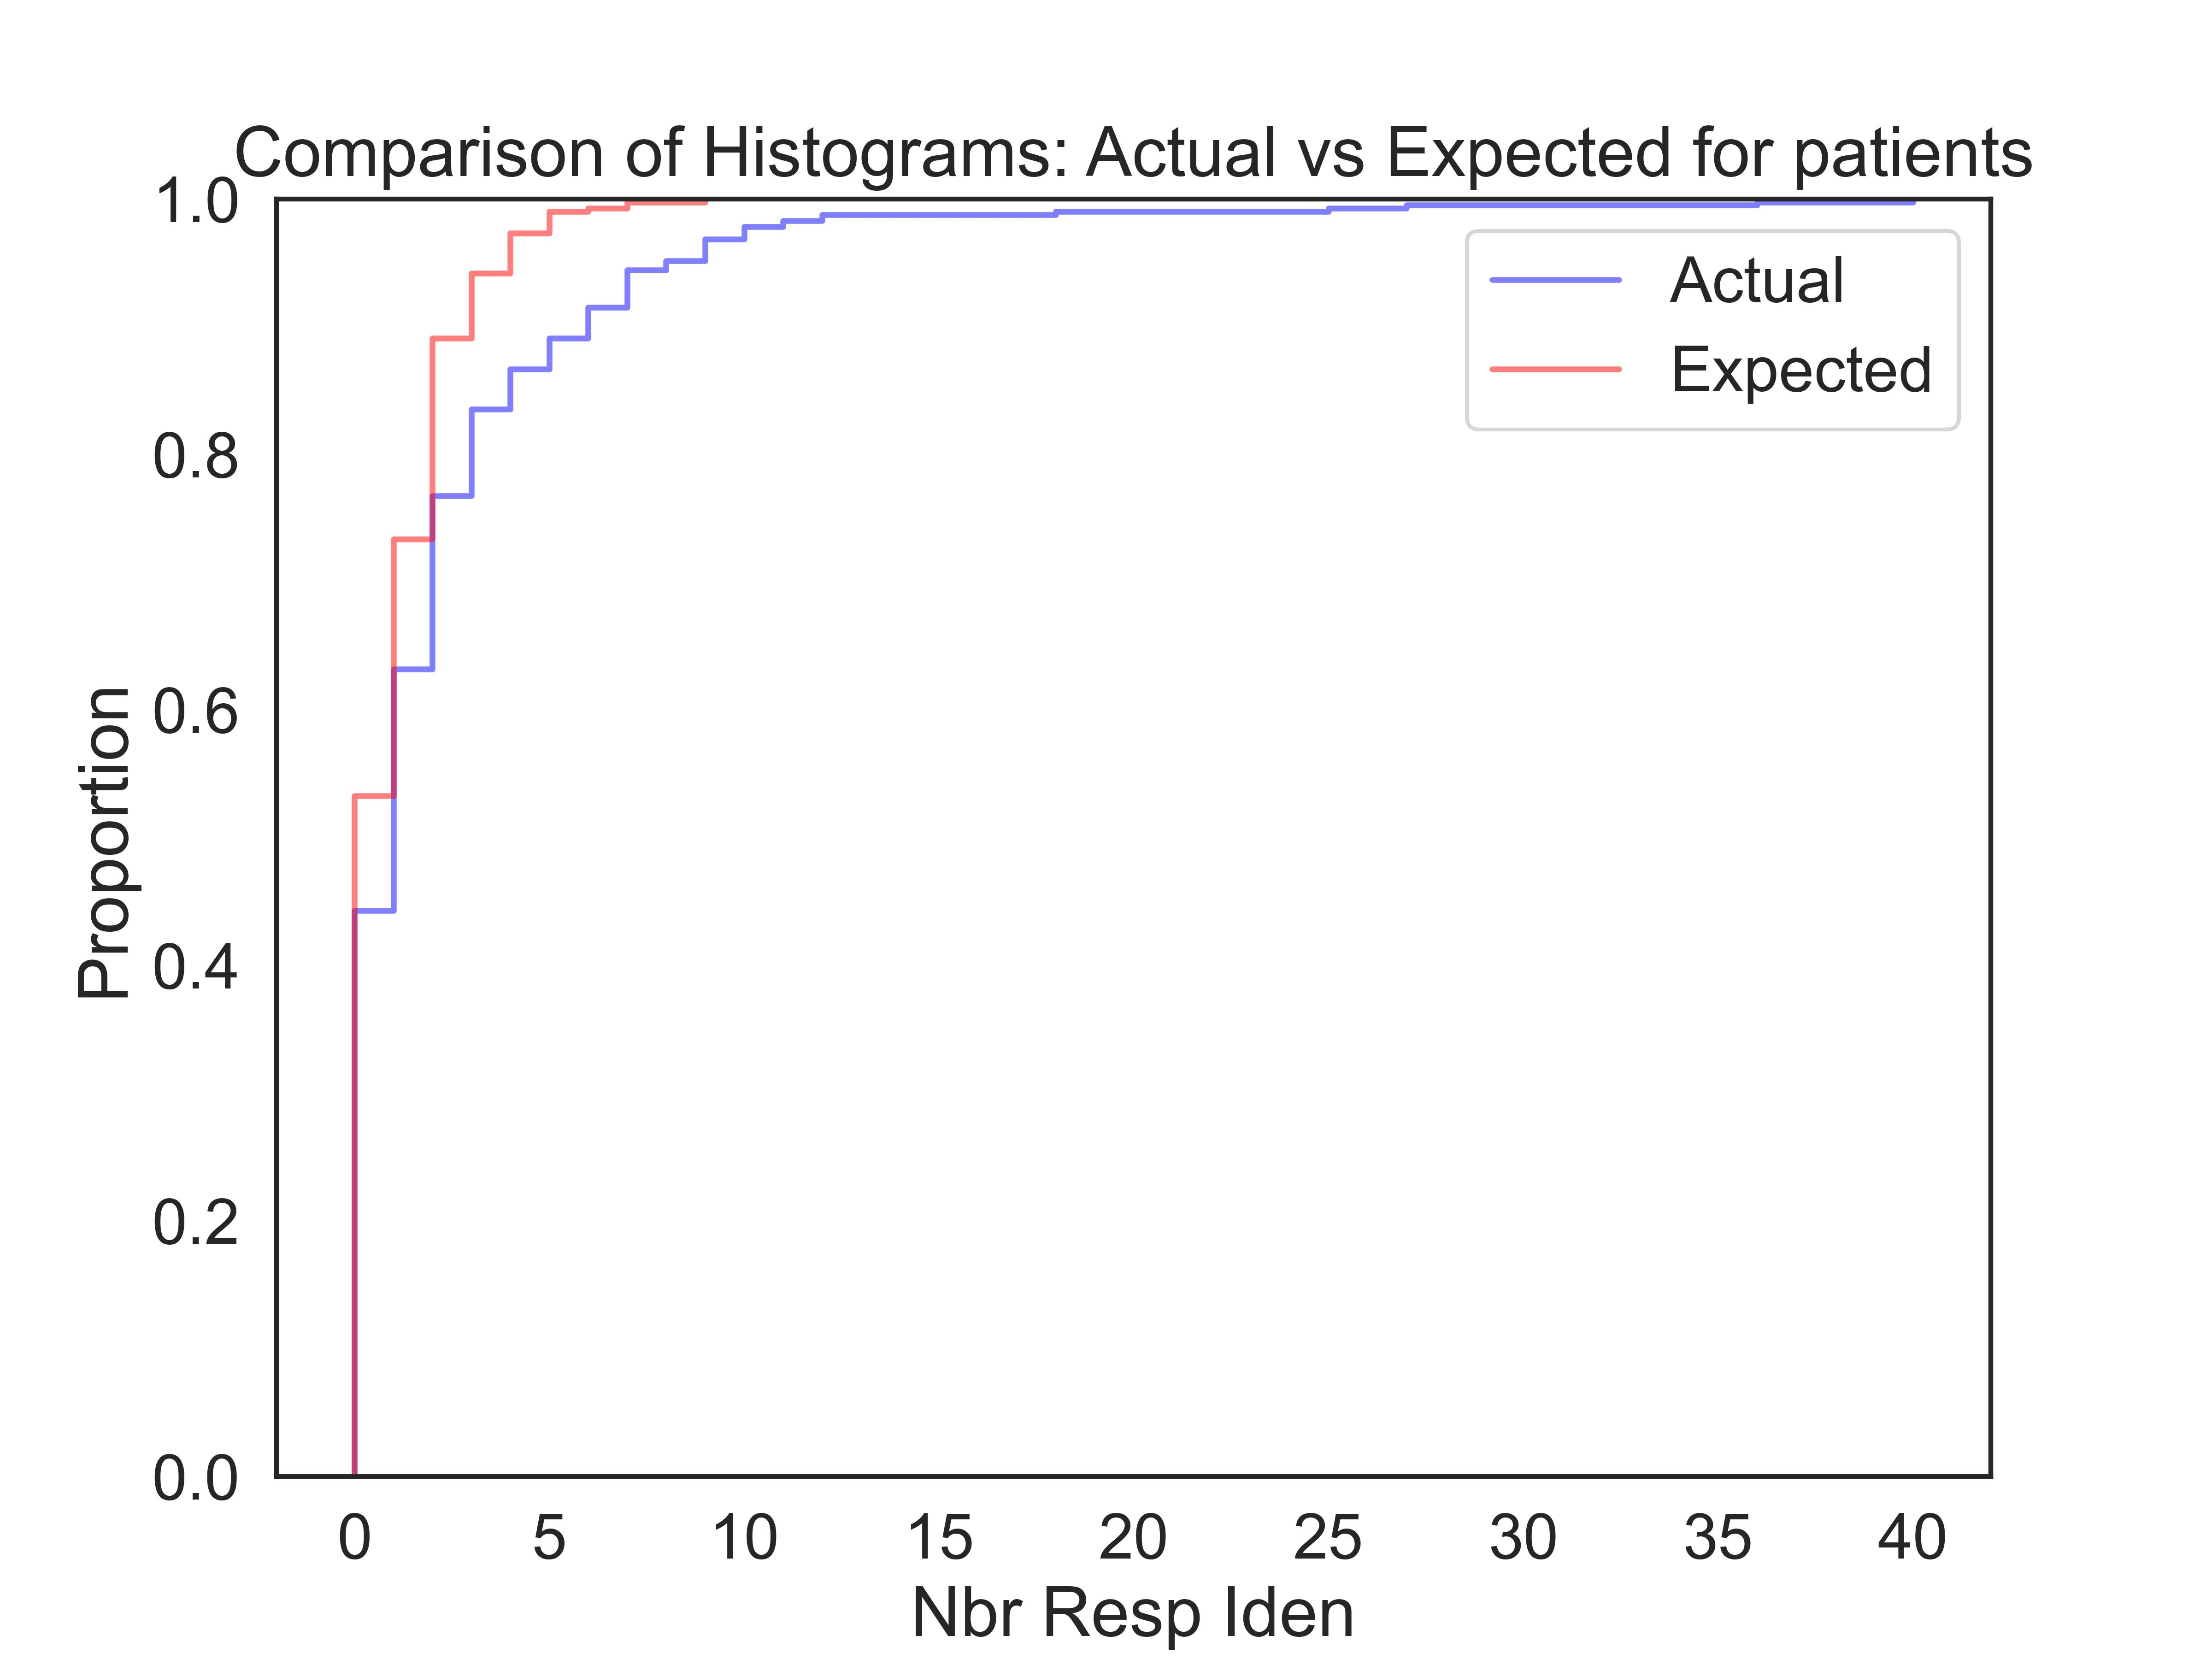
\includegraphics[width=12cm,height=7cm]{MainLayout/Images/chapter9/actual_expected_patients_ecdf.jpg}
    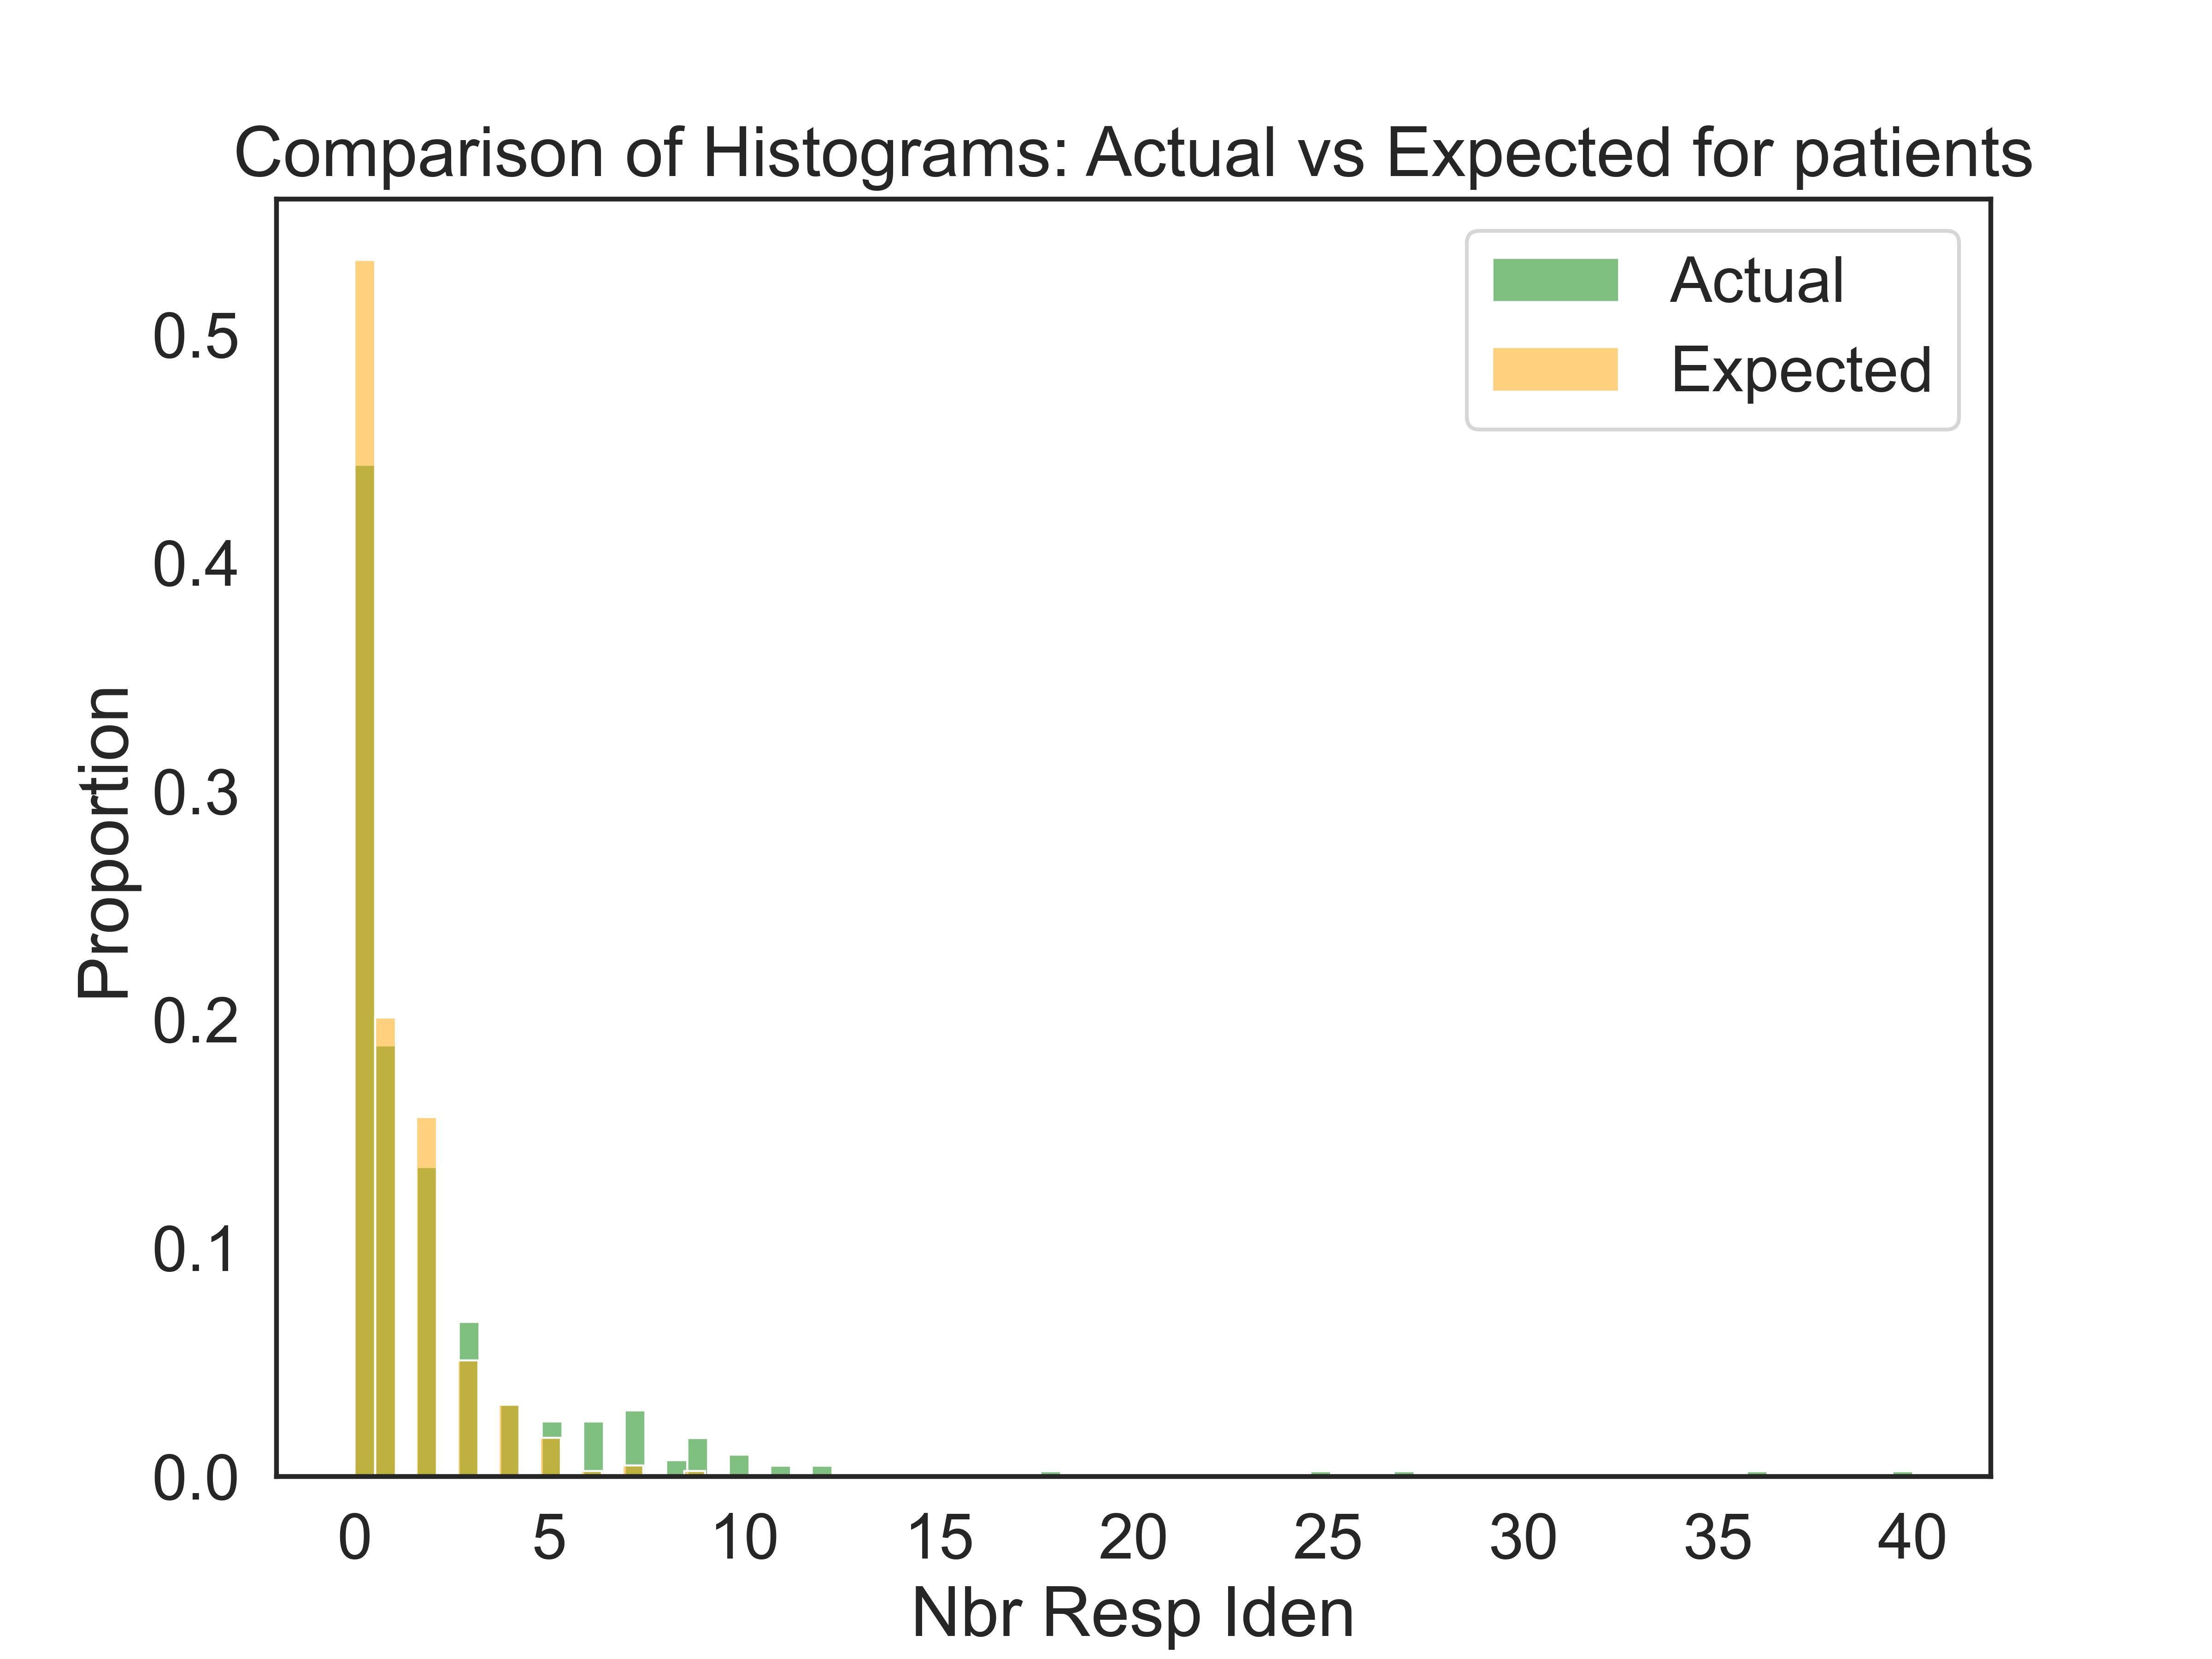
\includegraphics[width=12cm,height=7cm]{MainLayout/Images/chapter9/actual_expected_patients_hist.jpg}
    \caption{Main Title for First Image \\ \small Subtitle for the first graphic.}
    \label{fig:actual_expected_patients}
\end{figure}

\section{Trial difficulty} 
One of the parameters we investigated for its potential effect on state transitions was trial difficulty, measured as the alignment between the stimulus difference and the participant’s engaged kernel. Specifically, we examined whether trial difficulty influences the likelihood of a participant transitioning from the engaged state to the perseverative state.

To assess this, we compared the distributions of trial difficulty between engaged trials that remained engaged and engaged trials that transitioned to perseveration. Unlike the number of consecutive identical responses, which depends on previous trials, trial difficulty is independent across successive trials, making this comparison more straightforward.

The results show no significant difference in trial difficulty between trials where participants transitioned to perseveration and those where they remained engaged (p=0.16). This suggests that perseveration is not directly driven by stimulus difficulty. If trial difficulty were a key factor, we would expect participants to transition into perseveration more frequently in harder trials. However, since no such effect is observed, it implies that internal cognitive processes, response biases, or fatigue may play a greater role in state transitions than trial difficulty alone.
\begin{figure}[H]
    \centering
    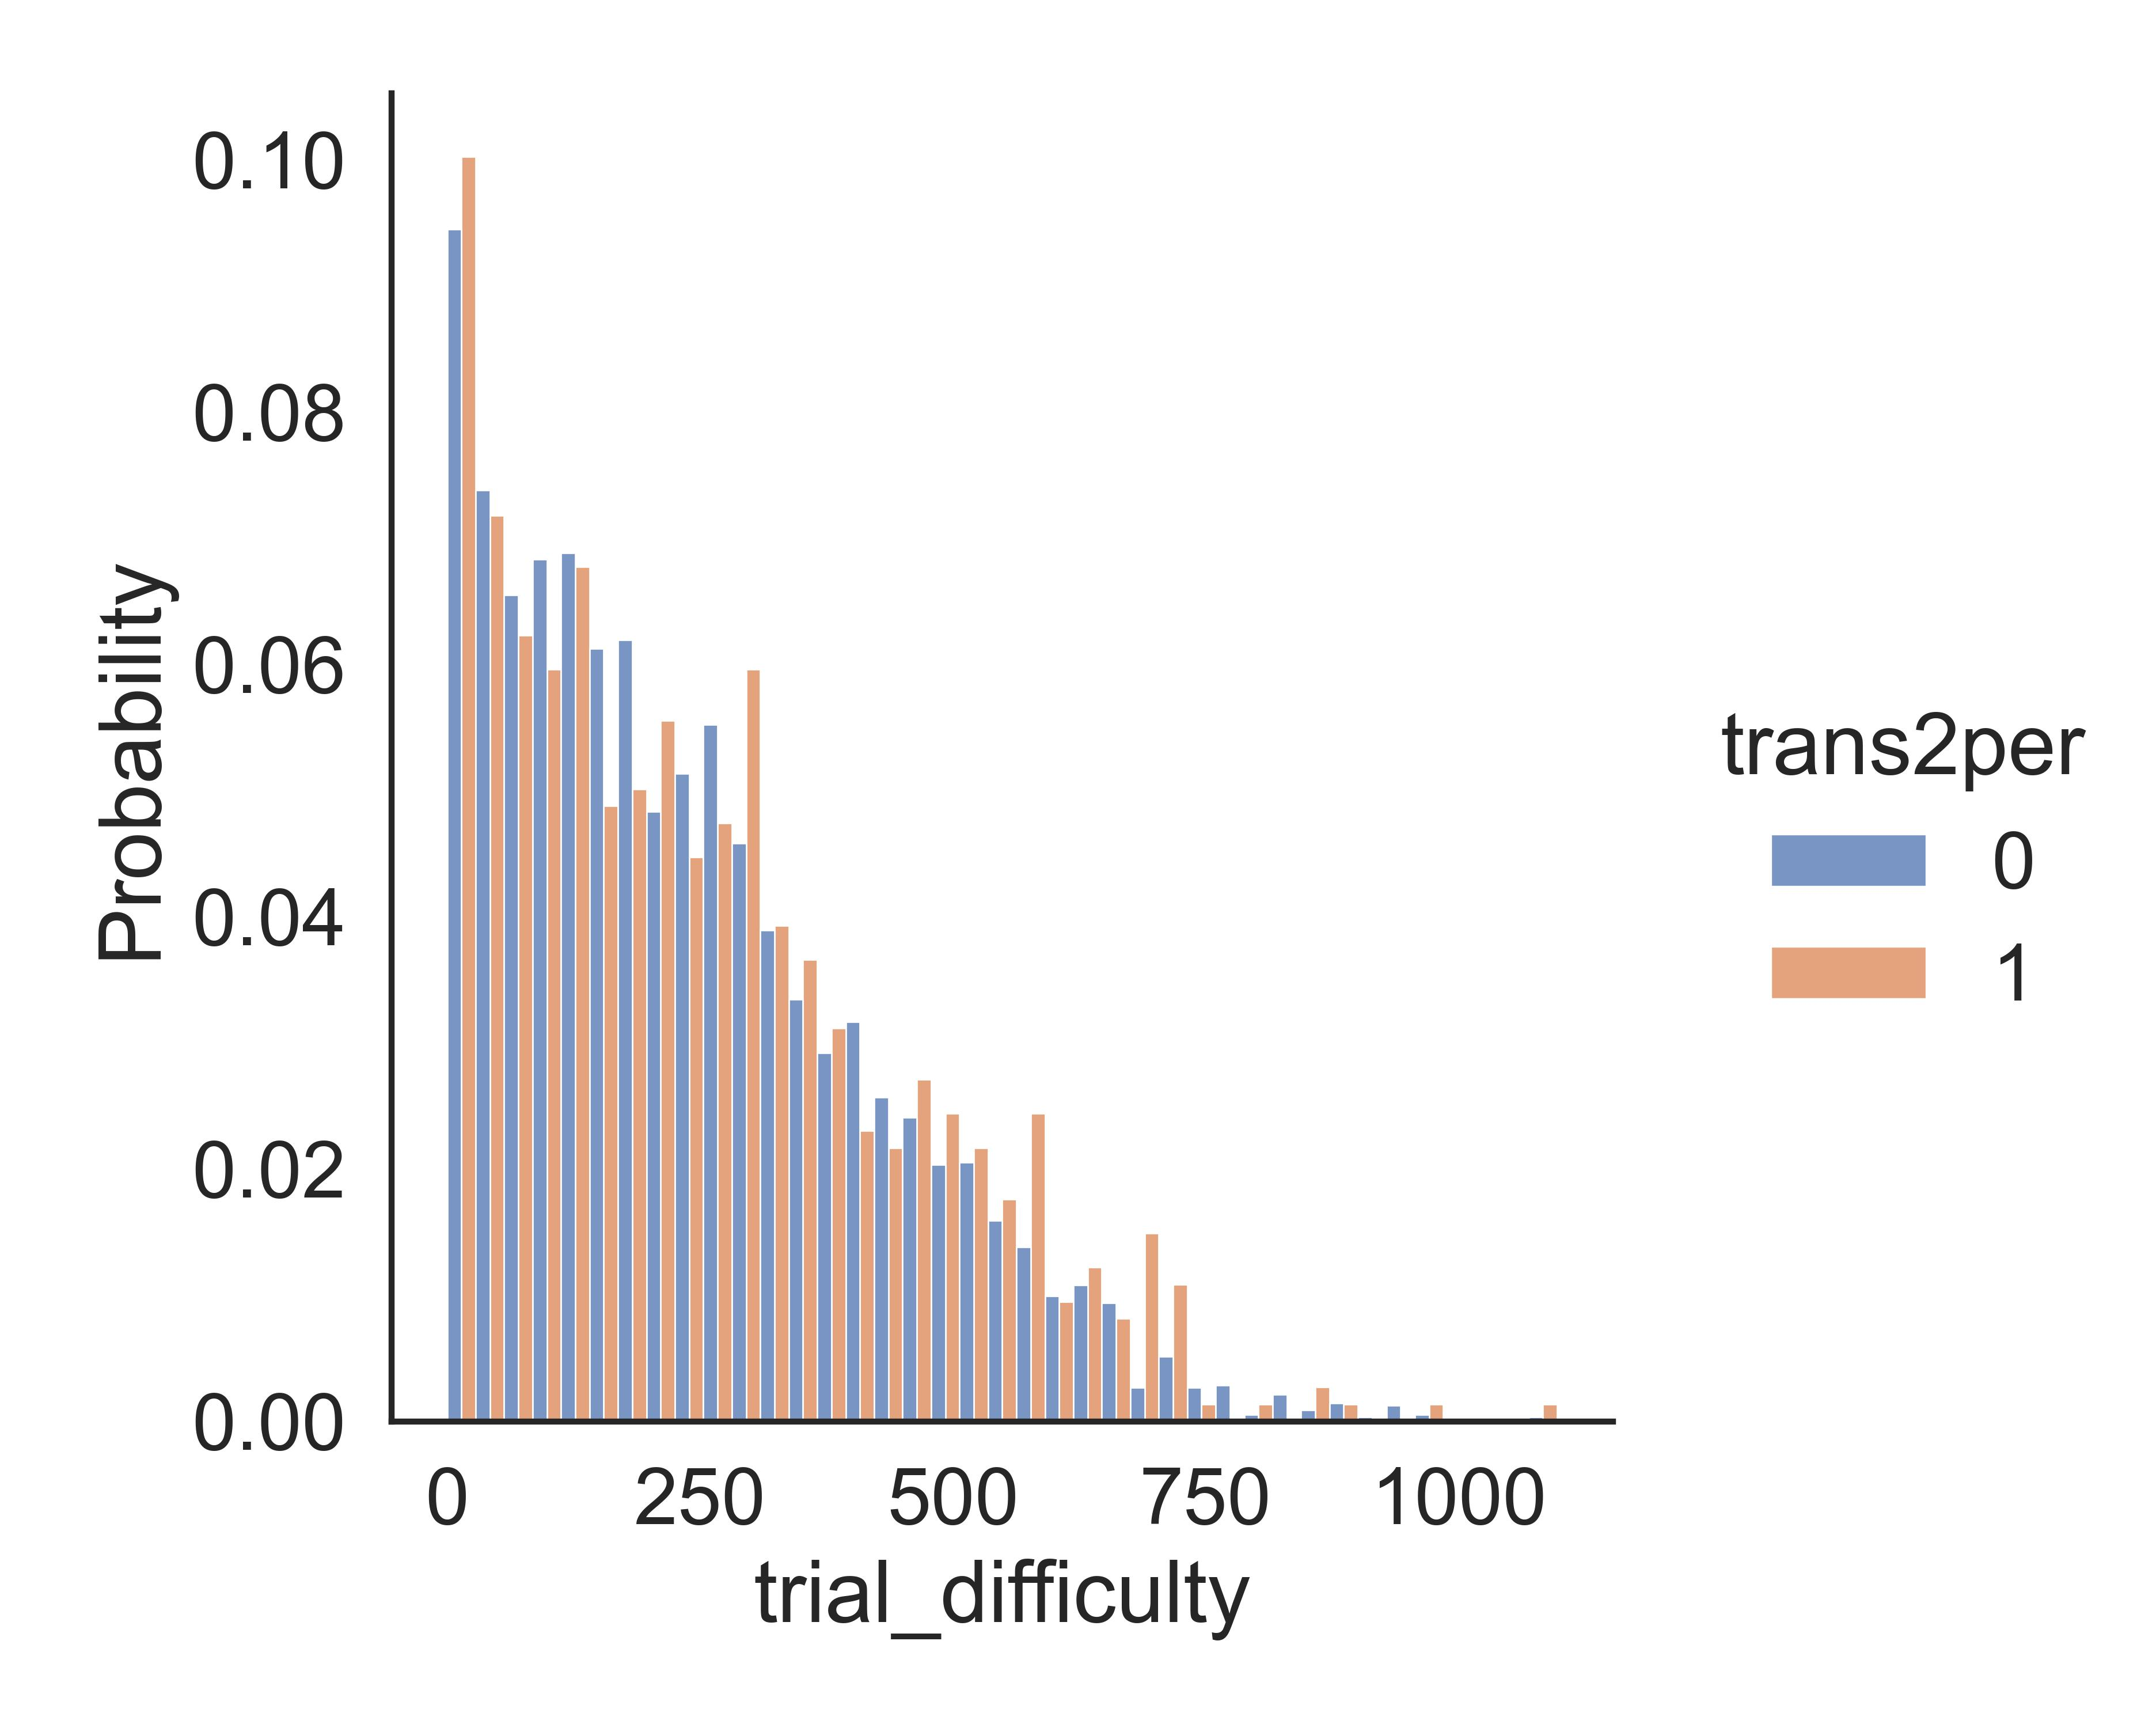
\includegraphics[width=12cm,height=7cm]{MainLayout/Images/chapter9/trial_difficulty.jpg}
    \caption{Main Title for First Image \\ \small Subtitle for the first graphic.}
    \label{fig:trial_difficulty}
\end{figure}


